\begin{table*}[t!]
\resizebox{\linewidth}{!}{
\begin{tabular}{lcllll||llll}
\toprule
& & \multicolumn{4}{c}{\textbf{Charades-STA}} & \multicolumn{4}{c}{\textbf{ActivityNet-Captions}} \\
\cmidrule(lr){3-6} \cmidrule(lr){7-10}
\textbf{Approach} & \textbf{Supervision} & \textbf{R@0.3} & \textbf{R@0.5} & \textbf{R@0.7} & \textbf{mIoU} & \textbf{R@0.3} & \textbf{R@0.5} & \textbf{R@0.7} & \textbf{mIoU} \\ \midrule
CTRL~\cite{Gao_2017_ICCV} & \multirow{2}{*}{Full} & - & 21.42 & 7.15 & - & 28.70 & 14.00 & - & 20.54 \\
LGI~\cite{mun_local-global_2020} & & 72.96 & 59.46 & 35.48 & 51.38 & 58.52 & 41.51 & 23.07 & 41.13 \\
\midrule
TGA~\cite{mithun_weakly_2019} & \multirow{5}{*}{Weak} & 29.68 & 17.04 & 6.93 & - & - & - & - & - \\
WSTG~\cite{chen_look_2020} & & 39.80 & 27.30 & 12.90 & 27.30 & 44.30 & 23.60 & - & 32.20 \\
SCN~\cite{lin_weakly-supervised_2020} & & 42.96 & 23.58 & 9.97 & - & 47.23 & 29.22 & - & - \\
WS-DEC~\cite{duan2018weakly} & & - & - & - & - & 41.98 & 23.34 & - & 28.23 \\
WSLLN~\cite{gao2019wslln} & & - & - & - & - & 42.80 & 22.70 & - & 32.20 \\
\midrule
PSVL$^{\dagger}$~\cite{nam_zero-shot_2021} & \multirow{4}{*}{None} & 46.63 & 30.84 & 13.57 & 31.09 & 43.03 & 25.14 & 10.96 & 30.77 \\
LFVL$^{\dagger}$~\cite{kim2023language} & & \underline{49.50} & \underline{34.39} & \underline{16.95} & \textbf{33.19} & 43.34 & 25.17 & \textbf{13.10} & \textbf{31.67} \\
\textbf{\modelname} & & {49.21} & \textbf{34.60} & \textbf{17.93} & {{32.73}} & {\textbf{46.05}} & {\underline{28.19}} & \underline{12.84} & \underline{31.11} \\
\textbf{\modelname$_{250}$} & & {\textbf{50.98}} & {{33.18}} & {{16.48}} & \underline{33.06} & \underline{45.43} & \textbf{28.27} & 12.81 &{30.88} \\
\bottomrule
\end{tabular}
}
\caption{Localization accuracy compared to zero-shot, weakly and fully supervised baselines. $^{\dagger}$ indicates reproduction with official checkpoints and/or implementations. The best-performing method is highlighted in bold and the second-best is underlined.}
\label{tab:resultsCompare}
\end{table*}
\section{Experiments}

\paragraph{Experimental Setup.}
Consistent with prior zero-shot NLVL research, we evaluate on Charades-STA \cite{Gao_2017_ICCV} and ActivityNet-Captions \cite{heilbron2015activitynet,krishna2017dense}. Note that we only utilize the video components of the dataset during training. Query and video span annotations are only used for evaluation purposes. We compare \modelname against several zero-shot \cite{nam_zero-shot_2021,kim2023language}, weakly supervised \cite{mithun_weakly_2019,chen_look_2020,lin_weakly-supervised_2020,duan2018weakly,gao2019wslln} and fully supervised~\cite{Gao_2017_ICCV,mun_local-global_2020} baselines. We evaluate performance with the mean temporal Intersection over Union (\textit{mIoU}) for the predicted video moment spans and recall at specific threshold values (\textit{R@k}), that is defined as the percentage of video span predictions with IoU value of at least \(k\), where \(k= \left\{ 0.3,0.5,0.7\right\} \), following prior works. 

\subsection{Experimental Results}
Table \ref{tab:resultsCompare} illustrates a comparative analysis of \modelname against baselines. We compare \modelname using two  \(G_{C}\) versions with varying the number of concepts in the commonsense module, \ie \(n_C \in \{300, 250\}\). We represent these configurations as \modelname and \modelname$_{250}$, respectively. 
\modelname outperforms the fully supervised CTRL baseline and all of the weakly supervised baselines by significant margins. In addition, \modelname surpasses the PSVL zero-shot baseline across various configurations, with a particularly strong performance in the higher recall regime (\(R@0.7\)).
For instance, for the Charades-STA dataset, \modelname consistently outperforms PSVL, yielding gains of up to $32.13\%$ in higher recall scenarios. Similarly, on the same dataset, \modelname achieves recall enhancements of up to $5.78\%$ over LFVL for \(R@0.7\). In the context of the ActivityNet-Captions dataset, \modelname also outperforms PSVL across all metrics, showcasing performance improvements ranging from $7.02\%$ to $17.15\%$.
Notably, \modelname substantially outperforms LFVL on ActivityNet-Captions in terms of \(R@0.3\) and \(R@0.5\) (up to $12\%$ for \(R@0.5\)), while maintaining comparable results in terms of \(R@0.7\) and \(mIoU\). Considering that ActivityNet-Captions represents a challenging benchmark encompassing diverse video themes, our findings highlight that leveraging commonsense information effectively helps integrate diverse visual-linguistic themes, outperforming methods that rely on pre-trained large-scale vision-language models.

Furthermore, since \(mIoU\) for all models is close to 30\%, an increase in  \(mIoU\) corresponds to a proportional increase in model predictions with recall above 0.3 (\(R@0.3\)).
The performance of \modelname with lower \vs higher $G_{C}$ sizes highlights a pattern of exclusivity between overall localization performance (\ie, \(mIoU\)) and precision of accuracy (higher recall regimes, \eg, \(R@0.7\)). This dichotomy between better recall at higher regimes and increased average localization highlights the trade-off between being able to generalize to a diverse set of videos and accurately localizing the moment in a specific video. Higher concept set sizes may provide wider levels of information to accommodate different types of videos better, but may impede the model's capability to ground the exact video moment accurately. 

\begin{wraptable}{r}{8cm}
\centering
\resizebox{0.6\textwidth}{!}{
\begin{tabular}{lrrrr}
\toprule
\textbf{Relations} & \multicolumn{1}{l}{\textbf{R@0.3}} & \multicolumn{1}{l}{\textbf{R@0.5}} & \multicolumn{1}{l}{\textbf{R@0.7}} & \multicolumn{1}{l}{\textbf{mIoU}} \\ \midrule
\textbf{S}         & 39.63                              & 26.53                              & 11.81                              & 26.03                             \\
\textbf{T}         & 44.98                              & 28.08                              & 13.93                              & 29.63                             \\
\textbf{ST}        & 49.84                              & 30.35                              & 15.16                              & 32.38                             \\
\textbf{F}         & 49.21                              & 34.60                               & 17.93                              & 32.73                             \\
\textbf{F-ST}    &  47.98	& 29.26&	14.29&	30.77\\
\textbf{All}       & 49.42                              & 34.03                              & 17.99                              & 32.85   \\
\bottomrule
\end{tabular}}
\label{tab:ablationRelation}
\caption{\modelname with Spatial (\textbf{S}), Temporal (\textbf{T}), Spatial and Temporal (\textbf{ST}) relations, the customized set of Filtered relations (\textbf{F}) mentioned in Table \ref{tab:relations}, \textbf{F} without the spatial/temporal relations (\textbf{F-ST}) and \textbf{All} relation types.}
\end{wraptable}

\subsection{Ablation Studies}
\label{sec:ablation}
Comprehensive ablation studies, found in the appendix, provide further insights into the importance of commonsense in zero-shot NLVL. Specifically, we evaluate (1) the influence of various relation types, (2) the relative significance of commonsense in augmenting video or query features, (3) the potential usefulness of auxiliary commonsense information, and (4) the best approach for injecting commonsense. 

\begin{figure*}[t!]
    \centering
    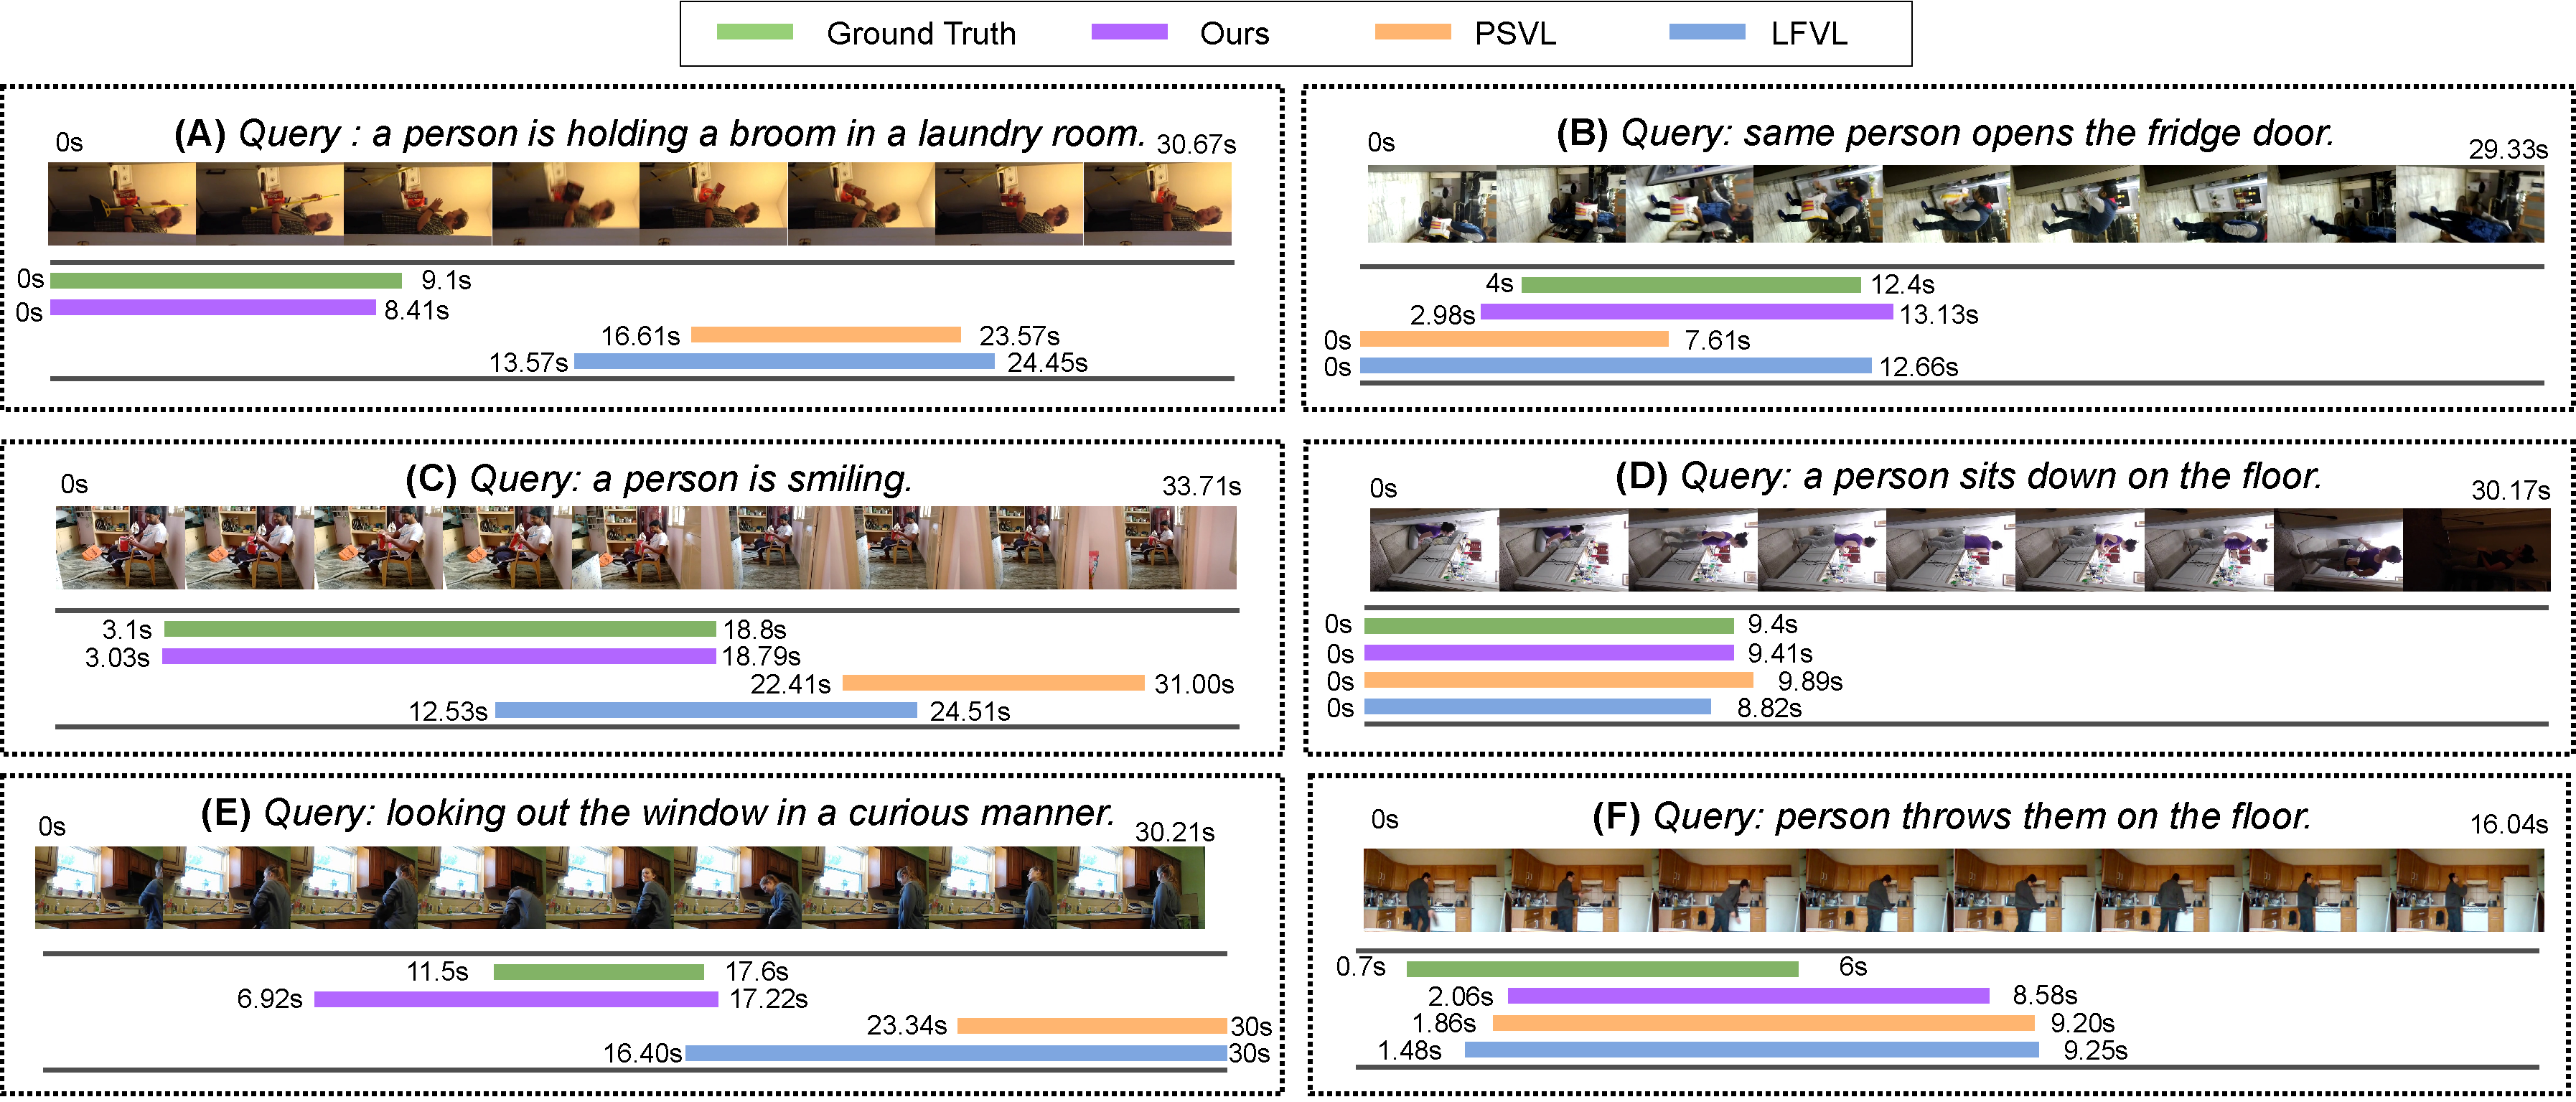
\includegraphics[width=.9\linewidth]{figures/figure_files/Qualitative.pdf}
  \caption{Qualitative inference results on examples from Charades-STA test data. Video span timestamps predicted by \modelname (\textcolor[HTML]{9900FF}{\textbf{purple}} lines), PSVL (\textcolor[HTML]{FF9900}{\textbf{orange}} lines), and LFVL (\textcolor[HTML]{7EA6E0}{\textbf{blue}} lines), juxtaposed with ground truth timestamps (\textcolor[HTML]{82B366}{\textbf{green}} lines).
  }
  \label{fig:qual}
\end{figure*}

\subsubsection{Which Relation Types Are Most Important?}
We analyze the contribution and relative importance of relation types used in building \(G_{C}\). Given that video localization requires spatiotemporal understanding, we hypothesize that relations falling in spatial/temporal categories are essential. Accordingly, we examine the performance of \modelname with 1) only spatial relations (\textbf{S}), 2) only temporal relations (\textbf{T}), and 3) both spatial and temporal relations (\textbf{ST}). We also evaluate \modelname with 4) a bigger subset of relations (as given in Table \ref{tab:relations}) to accommodate domain invariance (\textbf{F}), 5) the relation set mentioned in the previous configuration excluding spatial and temporal relation types (\textbf{F-ST}), and 6) all relations in ConceptNet (\textbf{All}). 

Table \ref{tab:ablationRelation} enumerates the results across all \modelname configurations. 
The performance drops significantly across all metrics with \textbf{S}, where only spatial relations are considered. The temporal relation set \textbf{T} performs much better than \textbf{S}, highlighting the higher importance of temporal commonsense than spatial commonsense for precise localization. Despite the poor recall performance on \textbf{S}, spatial relations are valuable to the localization process, which is supported by a further improved performance with \textbf{ST}, which considers both spatial and temporal relations. The considerable drop in performance of \textbf{F-ST}, a filtered set that excludes spatial and temporal relation types, as compared to \textbf{F} and \textbf{ST}, further emphasizes the importance of spatial and temporal commonsense information for accurate localization. 
Finally, performance is considerably high with all relations included (\textbf{All}), but not significantly better than previous configurations that use a far smaller $G_{C}$ and are hence more resource-efficient. Overall, \textbf{F} seems to provide a good balance between recall at various levels and mean localization accuracy. 

\section{Qualitative Results}
We present qualitative results w.r.t. \modelname's localization performance along with the PSVL and LFVL baselines. In Figure~\ref{fig:qual}, we showcase a few examples from the Charades-STA test split, accompanied by ground-truth video and query annotations and the localization results of the three models. Examples (A)-(C) show how \modelname accurately localizes the video moment, while PSVL and LFVL perform poorly. Upon inspection, PSVL and LFVL localize succeeding but semantically different events from the target segment in (A) and (C). 
On the other hand, in (B), PSVL and LFVL are seen to localize temporally preceding events along with the target event jointly. 
This example is challenging since the query includes ``same person", which requires the ability to contextualize and distinguish preceding events from the target event. The inability of PSVL and LFVL baselines to localize the target segment alone (\ie, isolating it from the preceding contextual segments), and conversely the accurate localization performance of \modelname, shows that \modelname can effectively contextualize and distinguish ``same person" as a co-referenced entity by leveraging commonsense. Our results corroborate previous works that demonstrate the usefulness of commonsense in co-reference resolution~\cite{coref_commonsense_ieee, coref_commonsense_acl_ravi-etal-2023-happens}. 

Example (D) highlights a case where all three models can localize accurately, while (E) and (F) show examples where none of the three models performs exceptionally well. However, it is important to note that \modelname localizes closest to the ground truth -- it captures the ground truth event, but also jointly localizes the preceding event, which is semantically similar to the target event, \ie, the person is looking outside the window. In contrast, PSVL and LFVL localize video segments that showcase events that are very distinct from the target query, \ie, the person in the frame is looking away from the window (\eg, LFVL localizes an event where the person is looking at the camera, whereas PSVL localizes the succeeding event where the person is looking down). Finally, all three models perform similarly in example (F). A deeper analysis reveals that each model localizes neighboring events in addition to the target event. 